\chapter{Выполнение работ по дозиметрическому и радиационному контролю} \label{chapt3}
\section{Программа производственного контроля} \label{sect3_1}
	В ходе производственной практики была проведена программа производственного 
	контроля на предприятии ЗАО <<Титан-Изотоп>>. Данные полученные в 
	ходе измерений представлены ниже.

	Территория предприятия была исследована на наличие радиационного загрязнения,
	составлена карта местности с нанесёнными на ней значениями радиационного фона  
	(данные представлены в мкР/час).

	\begin{figure}[ht]
		\centering
		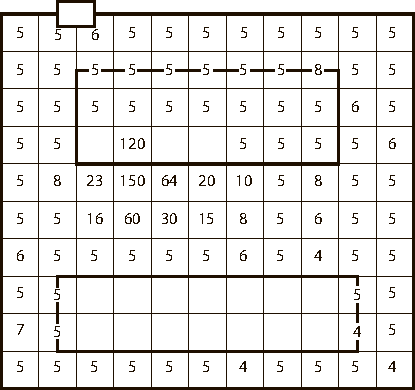
\includegraphics[width=0.5\textwidth]{nuclear_scheme.pdf}
		\caption{Территория предприятия}
	\end{figure}

	В целом на территории предприятия полученные значения соответствуют фоновым 
	(не превышают значения 50 мкР/час) за исключением стационарного хранилища 
	радиоактивных веществ, где значения не превышают 1 мР/час, т.е. можно 
	вести работы вблизи хранилища без вреда для здоровья.

	\begin{table}[ht]
		\centering
		\caption{<<Горячая камера>>}
		\begin{tabular}{|p{4cm}|p{2.5cm}|p{3cm}|p{2.8cm}|p{2.5cm}|}
			\hline
			Объект & Вид & Контрольный уровень & Прибор & Результат \\ \hline
			Рабочее место у манипулятора в операторной & Измерение мощности дозы & 
				1 мкЗв/час & ДРГ-01Т1 МКС-01Р-01 & 0,08\( \pm \)0,04 мкЗв/час \\ \hline
			Захваты манипулятора, поверхности подвижного стола & Контроль р/а 
				загрязнённости методом мазков & Отсутствие снимаемых загрязнений &
				МКС-01Р-01 & отсутствует \\ \hline
		\end{tabular}
	\end{table}

	\begin{table}[ht]
		\centering
		\caption{Дозиметрическия градуировочныя установка УПГД}
		\begin{tabular}{|p{4cm}|p{2.5cm}|p{3cm}|p{2.8cm}|p{2.5cm}|}
			\hline
			Объект & Вид & Контрольный уровень & Прибор & Результат \\ \hline
			Рабочее место оператора при открытой заслонке установки УПГД на 2 
				высотах: 1,0 и 1,5 м над полом & Измерение мощности дозы & 
				2,0 мкЗв/час & ДРГ-01Т1 & 0,2 мкЗв/час 0,2 мкЗв/час \\ \hline
			Поверхность защитного блока с источниками линейки УПГД & 
				Измерение мощности дозы & 2,0 мкЗв/час & ДРГ-01Т1 & 
				0,04\( \pm \)0,01 мкЗв/час \\ \hline
			Поверхность сейфа с ИИИ & Измерение мощности дозы & 1 мкЗв/час & 
				ДРГ-01Т1 & 0,05\( \pm \)0,005 мкЗв/час \\ \hline
		\end{tabular}
	\end{table}

	\begin{table}[ht]
		\centering
		\caption{Стационарное хранилище радиоактивных веществ}
		\begin{tabular}{|p{4cm}|p{2.5cm}|p{3cm}|p{2.8cm}|p{2.5cm}|}
			\hline
			Объект & Вид & Контрольный уровень & Прибор & Результат \\ \hline
			Определение эквивалентной равновесной объёмной активности Радона-222 
				в помещениях подразделения ЗАО <<Титан-Изотоп>> & -- & 
				1000 Бк/м\(^3\) & РРА-01М-03 & 191,5\( \pm \)36,0 Бк/м\(^3\) \\ \hline
		\end{tabular}
	\end{table}

\clearpage
